\section{Case Study}
\label{sec:case_study}

\begin{figure}
	\begin{center}
		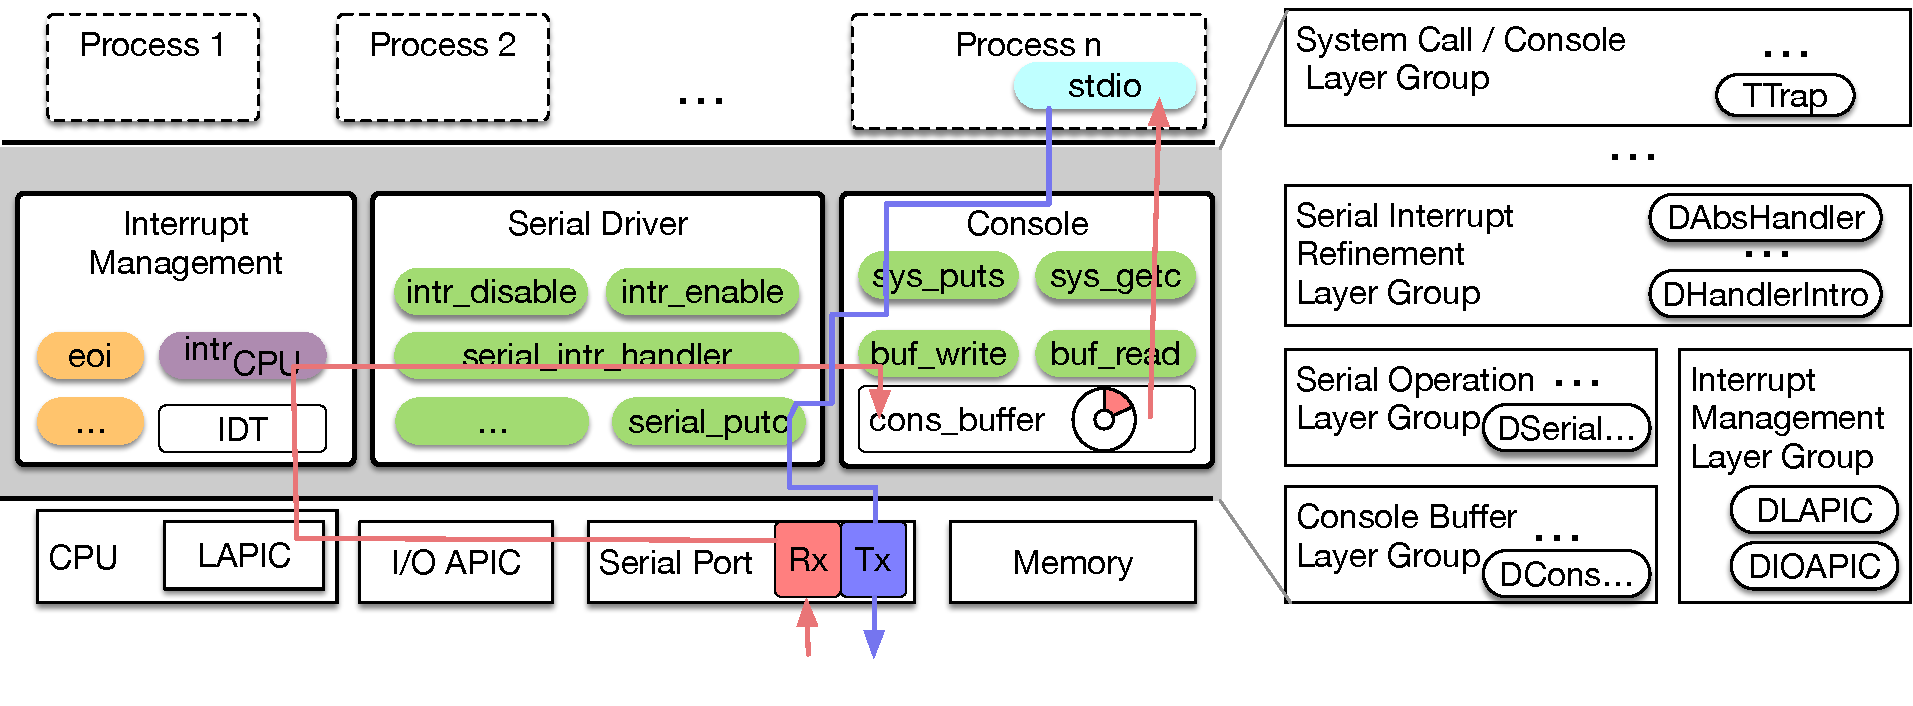
\includegraphics[scale=0.35]{figs/data_flow}
	\end{center}
	\caption{The data-flow of serial console messages and corresponding layer decomposition}
	\label{fig:data-flow}
\end{figure}


In this section, we present case studies of our verified drivers.
Fig.~\ref{fig:data-flow} shows the overall structure of our verified serial
console, while the left side reflects how the implementation of driver modules
organized as well as the data / control flow. The right side gives an overview
of how those modules are verified by construction of certified layers. We have
used a single controller in Sec.~\ref{sec:driver} to make the presentation
concise. However, mCertiKOS utilizes two physical interrupt controller devices:
the I/O Advanced Programmable Interrupt Controller (I/O APIC) and the Local
Advanced Programmable Interrupt Controller (Local APIC). Together with the
serial device, we present the formal models of these three hardware devices
throughout this section.

As shown in Fig.~\ref{fig:data-flow}, at the system call level, users can invoke
relevant system calls (\text{sys\_getc}, \text{sys\_puts}, {\it etc}) to read
from or write to the serial port. The red lines in the figure represents the
flow of receiving data from serial port. The implementation is interrupt driven.
Thus, when the serial receiving buffer (Rx) gets new data, the device triggers
an interrupt that goes through the Local APIC and I/O APIC devices and the
interrupt handler of serial device stores the data into the console circular
buffer (\texttt{cons\_buffer}). Later, when a user process makes the system call
\text{sys\_getc}, the system call handler simply pops and returns the head of
\texttt{cons\_buffer}. On the transmitting side, writing data to the serial port
(blue lines in the figure) is completely synchronous. When the system call
\texttt{sys\_puts} is invoked, the system call handler calls the transmission
function \texttt{serial\_putc} of serial driver to write data to the
transmission buffer (Tx) of serial device. The critical sections are protected
by the functions \texttt{serial\_intr\_disable} and
\texttt{serial\_intr\_disable} which masks and unmasks the interrupt signal of
the serial device.

The verification of the console circular buffer (\texttt{cons\_buffer}) is
already presented in Chapter \ref{chapter:framework}. In this section, we also present
the formal model and verification of their drivers for the serial port, I/O
APIC, and Local APIC.

\subsection{Serial Port}

Fig.~\ref{fig:serial} illustrates a typical serial port with a bounded internal
buffer of size 12. It consists of a RS-232 interface and a Universal
Asynchronous Receiver/Transmitter (UART) controller. RS-232 delivers electrical
signals between the UART controller and the connected cable. The UART controller
is responsible for demodulating received data into digital bits and storing them
into the internal receiving (Rx) buffer, and also modulating sent data from
digital bits and inserting them into the transmission (Tx) buffer.

The hardware UART controller has many features, and the mCertiKOS serial driver
only utilizes those parts needed for sending and receiving character strings.
When modeling the serial port, we take the minimalistic approach of only
modeling the set of features utilized by the existing drivers. The internal
state of the serial port device is defined as:

\begin{definition} \label{def:serial-device}
	Abstract state of serial device.
\[
\begin{array}{lll}
s = ( & \mathsf{RxBuf}: \mathsf{list} ~ \mathsf{char}, & \vartriangleright \textit{Receiving buffer} \\
 & \mathsf{TxBuf}: \mathsf{list} ~ \mathsf{char}, & \vartriangleright \textit{Transmission buffer} \\
 & \mathsf{irq}: \mathsf{bool}, & \vartriangleright \textit{Interrupt pending} \\
 & \mathsf{Connected}: \mathsf{bool}, & \vartriangleright \textit{Power} \\
 & \mathsf{Base}: \mathbb{Z}, & \vartriangleright \textit{Base address} \\
 & \multicolumn{2}{l} {\vartriangleright \textit{Line and modem configurations:}} \\
 & \multicolumn{2}{l}{\mathsf{RxIntEnable}: \mathsf{bool}, ~ \mathsf{DLAB}: \mathsf{bool}, ~ \mathsf{Baudrate}: \mathbb{Z},} \\
 & \multicolumn{2}{l}{\mathsf{Databits}: \mathbb{Z}, ~ \mathsf{Stopbits}: \mathbb{Z}, ~ \mathsf{Parity}: \mathsf{ParityType},} \\
 & \mathsf{FIFO}: \mathbb{Z}, ~ \mathsf{Modem}: \mathbb{Z} ~). \\
\end{array}
\]
\end{definition}
		
There are three external events for the serial device. The serial event
$\textsf{Recv}~ s$ indicates that a string has been received. The
$\textsf{SendingCompAck}$ event implies the device received the acknowledgment
that the characters in the transmission buffer have been sent out successfully,
while the $\textsf{NoSendingCompAck}$ events indicates that the sending of
characters in the transmission buffer is not yet complete.

The serial device is configured to trigger an interrupt when it receives data (a
nonempty string), and not to trigger any interrupt when the transmission buffer
becomes empty, i.e., when the characters in the transmission buffer are sent out
successfully. Thus, before any data is written to the serial port, we have to
poll the transmission status until it becomes empty. We have chosen this setup
because it covers both interrupt-triggering and polling events.

Note that, the states $s.\mathsf{RxBuf}$ and $s.\mathsf{irq}$ are disjoint from
$s.\mathsf{TxBuf}$ under the environment transitions in that the former is for
receiving data and the latter is for sending data only.  This allows us to use
two separate local logs in our device model, $\ell_{\textsf{tx}}$ (for
transmission) and $\ell_{\textsf{rx}}$ (for receiving), to handle these possibly
commutative events.

\begin{figure}
	\begin{center}
		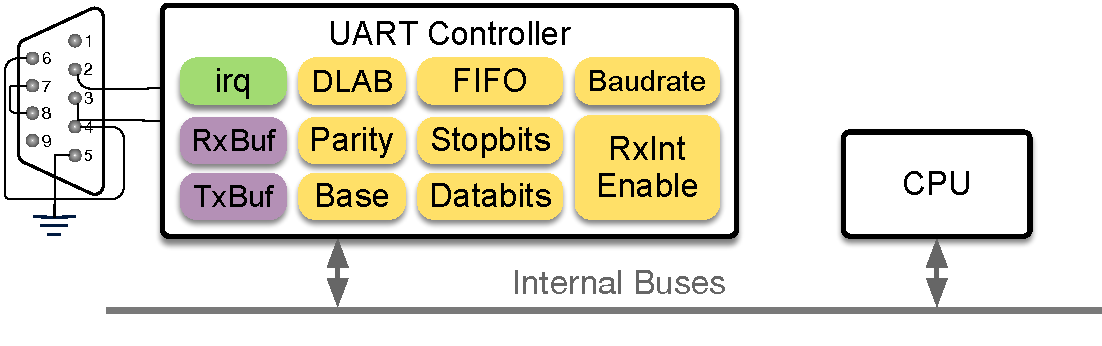
\includegraphics[scale=0.4]{figs/serial}
	\end{center}
	\caption{The hardware connections of a serial port}
	\label{fig:serial}
\end{figure}

\begin{figure}
\[
\begin{array}{cr}
	\inferrule{
		s.\mathsf{Connected} = \textsf{true} \\
		s.\mathsf{RxIntEnable} = \textsf{true} \\
		e = \mathsf{Recv} ~ w \\\\
		w \neq nil \\
		\textsf{newBuf} = \texttt{last}(\mathsf{BufSize}, (s.\mathsf{RxBuf} \textsf{++} w))
	}{
	  \delta^{\textsf{env}} (s, e) \defeq s[\mathsf{RxBuf} \leftarrow \textsf{newBuf}][\mathsf{irq} \leftarrow \textsf{true}]
	} & \text{(recvd\_irq)} \\[5ex]

	\inferrule{
	s.\mathsf{Connected} = \textsf{true} \\
	s.\mathsf{RxIntEnable} = \textsf{false} \\
	e = \mathsf{Recv} ~ w \\\\
	w \neq nil \\
	\textsf{newBuf} = \texttt{last}(\mathsf{BufSize}, (s.\mathsf{RxBuf} \textsf{++} w))
}{
	\delta^{\textsf{env}} (s, e) \defeq s[\mathsf{RxBuf} \leftarrow \textsf{newBuf}]
} & \text{(recvd\_no\_irq)} \\[5ex]

	\inferrule{
		s.\mathsf{Connected} = \textsf{true} \\
		e = \mathsf{Recv} ~ w \\
		w = nil 
	}{
		\delta^{\textsf{env}} (s, e) \defeq s
	} & \text{(norcv)} \\[5ex]

	\inferrule{
		s.\mathsf{Connected} = \textsf{true} ~~~~
		e = \mathsf{SendingCompAck} 
	}{
		\delta^{\textsf{env}} (s, e) \defeq s[\mathsf{TxBuf} \leftarrow \emptyset]
} & \text{(sent)} \\[5ex]

	\inferrule{
		s.\mathsf{Connected} = \textsf{true} ~~~~
		e = \mathsf{NoSendingCompAck} 
	}{
		\delta^{\textsf{env}} (s, e) \defeq s
} & \text{(noack)} \\[5ex]

	\inferrule{
		s.\mathsf{Connected} = \textsf{true} \\
		o = \textsf{input} ~ n \\\\
		n = s.\mathsf{Base} + 0 ~~~~
		s.\mathsf{DLAB} = \textsf{false} ~~~~
		s.\mathsf{RxBuf} = w \\
	}{
		\delta^{\textsf{CPU}} (s, o) \defeq s[\mathsf{RxBuf} \leftarrow \texttt{tl} ~ w ][\mathsf{irq} \leftarrow \textsf{false}] 
        } & \text{(read)} \\[5ex]
        
\inferrule{
	s.\mathsf{Connected} = \textsf{true} \\
	o = \textsf{output} ~ n ~ v\\\\
	n = s.\mathsf{Base} + 0 ~~~~
	s.\mathsf{DLAB} = \textsf{false} ~~~~
	s.\mathsf{TxBuf} = w \\
	}{\delta^{\textsf{CPU}} (s, o) \defeq s[\mathsf{TxBuf} \leftarrow \texttt{last}(\mathsf{BufSize}, (w \textsf{++} [v]))]\hspace*{-0.05in}
	} & \text{(write)} \\[5ex]

\inferrule{
	s.\mathsf{Connected} = \textsf{true} \\
	o = \textsf{output} ~ n ~ v\\\\
	n = s.\mathsf{Base} + 0 ~~~~
	s.\mathsf{DLAB} = \textsf{true} ~~~~
	r = (s.\mathsf{Baudrate}~\&~\mathsf{0xff00})~|~v \\
}{\delta^{\textsf{CPU}} (s, o) \defeq s[\mathsf{Baudrate} \leftarrow r]} & \text{(baudrate\_low)}
\end{array}
\]
\caption{The environment and CPU transition functions}
\label{fig:env-cpu-trans}
\end{figure}

Next, in Fig.~\ref{fig:env-cpu-trans}, we define the transition functions
$\delta^{\textsf{env}}$ and $\delta^{\textsf{CPU}}$, where
$\delta^{\textsf{env}}$ needs to handle all the possible environmental events
against the current state, and $\delta^{\textsf{CPU}}$ updates the current state
based on the input and output addresses and values. Note that function
\texttt{last} is used to model the action of dropping some elements in the front
of the buffer when the length of the new buffer exceeds the hardware buffer size
($\mathsf{BufSize}$). The \textsf{baud\_low} in Fig.~\ref{fig:env-cpu-trans} is an
example configuration of the control registers. The value of
\textsf{Baudrate} is not used to simulate the timing of the signal, but
is checked against the real hardware settings in certain transitions, such
as $\delta^{\textsf{CPU}}$ for \textsf{read} and \textsf{write}, in order to
verify that the driver is free of mis-configuration bugs.

% The following rules exhibit some interesting transitions.

By instantiating the device state and transition functions from our general
device model in Sec.~\ref{sec:model}, we create a concrete model of the serial
port with the \texttt{read} and \texttt{write} primitives.

\begin{figure}
	\lstinputlisting [language=C, multicols=2] {src/serial_putc.c}
	\caption{The implementation of \texttt{serial\_putc} and \texttt{serial\_getc} in C}
	\label{fig:serial_putc}
	\vspace{-10pt}
\end{figure}

Next, we show how the drivers are specified and verified on top of this model.
Fig.~\ref{fig:serial_putc} shows code fragments of the function
\texttt{serial\_putc} and \texttt{serial\_getc}.  There, the
\texttt{serial\_read} and \texttt{serial\_write} are the two primitives in the
serial hardware model, while \texttt{get\_serial\_exist} is a new primitive (already
verified in some underlay) indicating whether the serial device is already
initialized. The if statement (line 3) prevents any misuse of
\texttt{serial\_putc()} before initialization.

For \texttt{serial\_putc}, if the $s.\textsf{TxBuf}$ buffer is initially empty,
or the device receives a $\textsf{SendingCompAck}$ event during the loop (line
4-6), the program sends the character \texttt{c} to the serial port (line 8).
The function \texttt{serial\_putc} is specified as follows:
\[
	\inferrule{
		s.\mathsf{TxBuf} = \emptyset \\
		s.\mathsf{get\_serial\_exist} = \textsf{true} \\\\
		s' = s[\mathsf{TxBuf} \leftarrow [c]] \\
		(e, \ell'_{\textsf{tx}}) = \texttt{next}(\ell^{env}, \ell_{\textsf{tx}}) \\
		(e', \ell''_{\textsf{tx}}) = \texttt{next}(\ell^{env}, \ell'_{\textsf{tx}})
	}{
	\texttt{serial\_putc} (s, c, \ell_{\textsf{tx}}, \ell^{env}) \defeq (s', \ell''_{\textsf{tx}})
	}
\]
\[
\inferrule{
	s.\mathsf{TxBuf} \neq \emptyset \\
	s.\mathsf{get\_serial\_exist} = \textsf{true} \\
	(e, \ell'_{\textsf{tx}}) = \texttt{next}(\ell^{env}, \ell_{\textsf{tx}}) \\
	s' = \delta^{env}(s, e) \\
	(s'', \ell''_{\textsf{tx}}) = \texttt{serial\_putc} (s', c, \ell'_{\textsf{tx}}, \ell^{env}) \\
}{
\texttt{serial\_putc} (s, c, \ell_{\textsf{tx}}, \ell^{env}) \defeq (s'', \ell''_{\textsf{tx}})
}
\]

The first rule above shows the case when the transmission buffer is
originally empty. Here, $\textsf{lsr}$ immediately becomes $1$ in the
first loop iteration, and the character is written to the transmission
buffer in the device right away. Note that the function \textsf{next}
is called twice because the implementation of \textsf{serial\_putc} has
two serial I/O operations for the base case: one to check whether the
transmission buffer is empty, and the other to put the
character into the transmission buffer. 

The second rule above shows the case when the initial transmission buffer
is not empty. Here, the device performs transition based on
the received event $e$, and repeats the same process until it finally
receives the $\textsf{SendingCompAck}$ event. Then, by definition of
$\delta^{env}$ in Fig.~\ref{fig:env-cpu-trans}, the transmission
buffer becomes empty and the next recursive call falls into the first
case of the specification.

As for \texttt{serial\_getc}, a check of status register will be first performed
to clear the \textsf{irq} state, and confirm that there are pending receiving
messages (line 16). If the receiving buffer is not empty, the head of the buffer is
fetched (line 17) and inserted into the console buffer.

\begin{figure}
	\lstinputlisting [language=C] {src/serial_puts.c}
	\caption{The implementation of \texttt{serial\_puts} in C}
	\label{fig:serial_puts}
	\vspace{-10pt}
\end{figure}

In Fig.~\ref{fig:serial_puts}, we show the implementation of the
driver function $\textsf{serial\_puts}$ that writes a string into the
serial device by repeatedly calling $\textsf{serial\_putc}$ for each
character in the input string. Each call to $\textsf{serial\_putc}$ is
wrapped with calls to $\textsf{serial\_intr\_disable}$ and
$\textsf{serial\_intr\_enable}$ (both derived from those
in Fig.~\ref{fig:intr-transition}) to protect the critical section.

\ignore{
Most of our drivers are implemented in ClightX~\cite{dscal15}, which
is an extension of the CompCert Clight language \cite{leroy09} with
abstract states and primitives.}
For each driver function, we prove
that the concrete implementation satisfies its specification. Our
proof is termination-sensitive; we prove total correctness of each
function. In the case of \texttt{serial\_putc}, the maximum iteration
counter ($12800$) is used solely to enforce termination. We maintain
an invariant on $\ell^{env}$ that the serial port receives a
$\textsf{SendingCompAck}$ event within $12800$ times the
\texttt{delay()} function is called. This assumption is reasonable
because a sending operation that does not complete within this
time frame implies an underlying hardware failure.


%
%
%\begin{figure}
%	\begin{lstlisting}[language=C]
%void serial_intr_handler () {
%	int rx, t = 0;
%	while ((serial_read(0x3FD) & 0x01) && 
%			t < CONS_BUFF_SIZE) {
%		rx = serial_read(0x3F8);
%		cons_buf_write(rx);
%		t++;
%	}
%}
%\end{lstlisting}
%	\caption{The implementation of \texttt{serial\_intr\_handler} in C}
%	\label{fig:serial_intr_handler}
%\end{figure}


%%%%%%%%%%%%%%%%%%%%%%%%%%%%%%%%%%%%%%%%%%%%%%%%%%%%%%%%%%%%%%%%%%%%%%%%%%%%%
\begin{figure}
	\begin{center}
		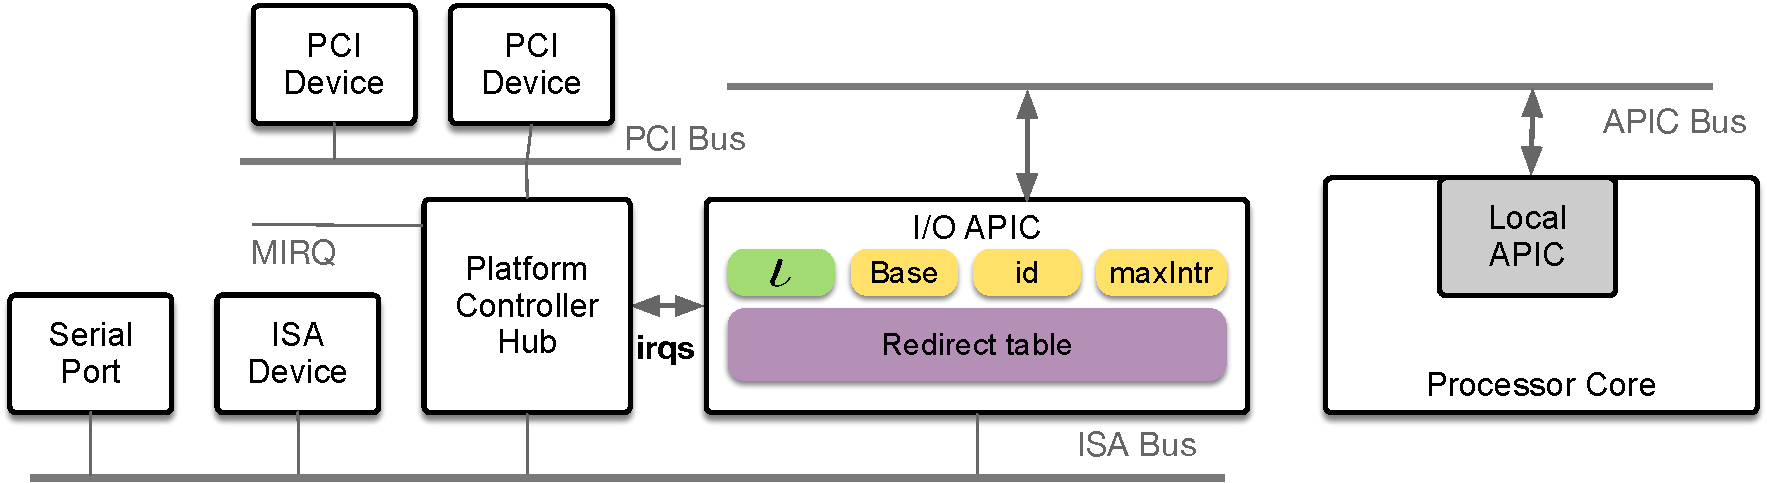
\includegraphics[scale=0.35]{figs/ioapic}
	\end{center}
	\caption{The hardware connections and registers of APIC}
	\label{fig:ioapic}
\end{figure}

\begin{figure}
	\begin{center}
	\[
	\begin{array}{lll}
	s = ( & \iota: \textsf{option} (\mathbb{Z} \times \mathbb{Z}), & \vartriangleright \textit{Current raised IRQ} \\
	& \textsf{id}: \mathbb{Z}, & \vartriangleright \textit{I/O APIC ID} \\
	& \textsf{maxIntr}: \mathbb{Z}, & \vartriangleright \textit{Max redirection entries} \\
	& \textsf{irqs}: \textsf{list} ~ \mathbb{Z}, & \vartriangleright \textit{Redirected IRQs} \\
	& \textsf{masks}: \textsf{list} ~ \textsf{TMask}, & \vartriangleright \textit{Interrupt line masks} \\
	& \textsf{dests}: \textsf{list} ~ \mathbb{Z}). & \vartriangleright \textit{Destinations in Local APIC ID} \\
	\end{array}
	\]
	\end{center}
	\caption{Internal states of I/O APIC}
	\label{fig:ioapic-states}
\end{figure}
%%%%%%%%%%%%%%%%%%%%%%%%%%%%%%%%%%%%%%%%%%%%%%%%%%%%%%%%%%%%%%%%%%%%%%%%%%%%%

\ignore{
The proof is achieved semi-automatically using the big-step semantics of the
CompCert Clight language. The automation is achieved through Coq tactic
libraries including the verification condition generator, arithmetic solvers,
various theory solvers (partial map, list, {\it etc}), and a number of domain
specific libraries which handle items such as device transitions and logs.  The
entire automation libraries are implemented in Coq's tactical language Ltac.
}

\subsection{I/O APIC}

An I/O APIC device collects interrupts from externally connected devices and
distributes them to the corresponding Local APIC. It can be programmed to mask
one or more of these interrupt lines, if the OS does not wish to receive
interrupts from some device(s).

Fig.~\ref{fig:ioapic} illustrates the registers and connections of an I/O APIC
device, which collects the IRQs from devices and route them to the Local APIC
controller on CPU. The ``redirect table'' controls the mapping between interrupt
lines and the IRQ number. Following our minimalistic approach, we omit logical
destination, remote-IRR configuration, and other features that are not used in
our kernel. The internal state of the I/O APIC is defined in
Fig.~\ref{fig:ioapic-states}, where $\iota$ represents the interrupt request
currently being processed and its corresponding destination LAPIC ID.

As an interrupt controller, the I/O APIC is treated as a special device. It does
not observe any event from the external environment, and thus has neither a
local log nor an environmental transition $\delta^{\textsf{env}}$, but instead,
it receives interrupt requests from the devices and EOI signals from the Local
APIC. We have introduced a special transition function $\delta^{intr}$ to
specify these interrupt-related behaviors.  Accordingly, $\delta^{intr}$ takes
two kinds of events: $\textsf{IRQ} ~ n$ indicates that an IRQ with number $n$ is
triggered by a device; and $\textsf{EOI}$ states that the latest interrupt
request has been handled by the OS.  The interesting parts of the transition
rules for $\delta^{intr}$ are shown in Fig.~\ref{fig:ioapic-transition}.

%%%%% Should we explain these rules? 

\begin{figure}
\begin{center}
\[\begin{array}{cr}
	\inferrule{
		s.\iota = \textsf{None} \\
		w = \textsf{IRQ} ~ n \\
		s.\textsf{irqs}[n] = q \\\\
		s.\textsf{masks}[n] = \textsf{Unmasked} \\
		s.\textsf{dests}[n] = d 
	}{
		\delta^{intr}(s, w) \defeq s[\iota \leftarrow \textsf{Some} ~ (q, d)] } & \text{(delivered)} \\[5ex]

	\inferrule{
		s.\iota = \textsf{None} \\
		w = \textsf{IRQ} ~ n \\
		s.\textsf{masks}[n] = \textsf{Masked} 
	}{
	\delta^{intr}(s, w) \defeq s 
} & \text{(masked)} \\[5ex]

\inferrule{
	s.\iota = \textsf{Some} (q, d) \\
	w = \textsf{EOI} \\
	s.\textsf{irqs}[n] = q \\
	s.\textsf{dests}[n] = d 
}{
\delta^{intr}(s, w) \defeq s[\iota \leftarrow \textsf{None}] 
} & \text{(EOI)} 
\end{array}
\]
	\end{center}
	\caption{I/O APIC transition rules}
	\label{fig:ioapic-transition}
\end{figure}

\begin{figure}
	\lstinputlisting [language=C, multicols=2] {src/ioapic.c}
	\caption{The implementation of \texttt{ioapic\_init} in C}
	\label{fig:ioapic_init}
\end{figure}

In addition to $\delta^{intr}$, the I/O APIC also contains the CPU transition
function $\delta^{\textsf{CPU}}$ used to specify the read/write primitives of
I/O APIC, discussed in Sec.~\ref{sec:model}.

In order to coordinate the IRQs assigned by the kernel with the external
interrupt vector, a kernel usually utilizes the Global System Interrupt (GSI)
number. Thus, the IC is first extended into a device object with this extra data
as part of its internal state. Then this IC object is further extended into more
abstract objects by introducing additional driver layers.

At the top level, the I/O APIC device object provides four primitives, two of
them are used to setup the IRQ mappings in the I/O APIC.  Specifically,
\texttt{ioapic\_init} initializes the device when the kernel boots, and
\texttt{ioapic\_enable} links a given interrupt line to a Local APIC when a new
device is plugged in or some device changes its working mode. Another two,
namely \texttt{ioapic\_mask} and \texttt{ioapic\_unmask}, are used to enable and
disable a certain interrupt line.

Function \texttt{ioapic\_init} in Fig.~\ref{fig:ioapic_init} shows the
initialization of the I/O APIC. It first reads the size of the interrupt
redirection table (line 2), and for each entry, marks the corresponding
interrupt to be edge-triggered, active high, and masked (i.e. not routed to any
Local APIC). The behavior of this function can be described using the following
rule:
\[
\inferrule{
	l = s.\mathsf{maxIntr} \\
	s' = s[\mathsf{masks}[1 .. l] \leftarrow \textsf{Masked}] \\ 
	s'' = s'[\mathsf{irqs}[1 .. l] \leftarrow \textsf{gsi} .. (\textsf{gsi}+l)][\mathsf{dest}[1 .. l] \leftarrow 0][\iota \leftarrow (\textsf{None}, \textsf{None})] \\
}{
	\texttt{ioapic\_init} (s) = s''
}
\]

Function \texttt{ioapic\_mask} in Fig.~\ref{fig:ioapic_init} shows the code for
masking interrupt line $n$. It first reads the entry `$n-\mathsf{gsi}$' in the
interrupt redirection table (line 13), sets the mask bit (line 14), and then
writes it back to the redirection table. The behavior can be described using the
following rule:
\[
\inferrule{
	\mathsf{gsi} \le n \le \mathsf{gsi} + s.\mathsf{maxIntr} \\ 
	s' = s[\mathsf{masks}[n - \mathsf{gsi}] \leftarrow \textsf{Masked}] \\
}{
	\texttt{ioapic\_mask} (s, n) = s'
}
\]

\subsection{Local APIC}

\begin{figure}
	\begin{center}
		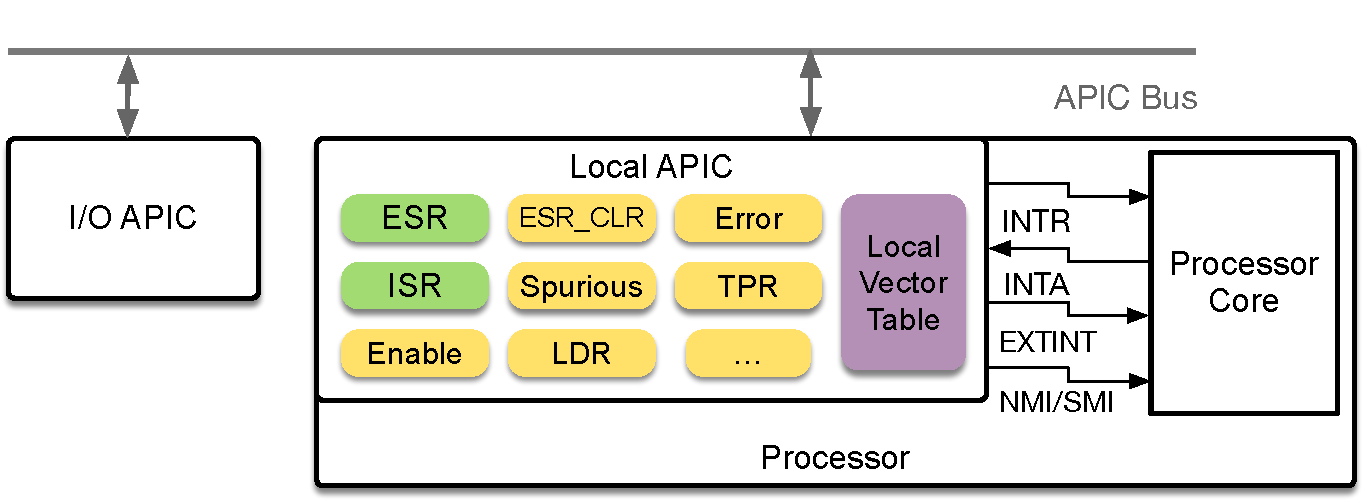
\includegraphics[scale=0.4]{figs/lapic}
	\end{center}
	\caption{The hardware connections of a Local APIC}
	\label{fig:lapic}
\end{figure}

Each processor has a Local APIC device which manages and delivers the interrupt
requests dedicated to this core. It serves as a bridge between I/O APIC and the
processor core and is also programmable which can be used to specify the manner
for each type of interrupt. As shown in Fig.~\ref{fig:lapic}, the Local APIC in
our kernel is mainly served to deliver the external interrupt and generate the
End-of-Interrupt (EOI) signals. An EOI signal indicates current interrupt is
completely handled so that the I/O APIC can issue the next interrupt.

\begin{figure}
	\begin{center}
		\[
		\begin{array}{lll}
		s = ( & \mathsf{ISR}: \textsf{option} (\textsf{IntType} \times \mathbb{Z}), & \vartriangleright \textit{Current in-service IRQ} \\
		& \textsf{ESR}: \mathbb{Z}, & \vartriangleright \textit{Error status register} \\
		& \textsf{ESR\_CLR}: \mathbb{Z}, & \vartriangleright \textit{ESR back-to-back clear ready} \\
		& \textsf{Enable}: \mathbb{B}, & \vartriangleright \textit{Local APIC enable} \\
		& \textsf{Spurious}: \mathbb{Z}, & \vartriangleright \textit{Spurious interrupt vector} \\
		& \textsf{Timer}: \textsf{LvtEntry}, & \vartriangleright \textit{Interrupt control of timer} \\
		& \textsf{Lint~0}: \textsf{LvtEntry}, & \vartriangleright \textit{Interrupt control of local connected I/O devices on line 0} \\
		& \textsf{Lint~1}: \textsf{LvtEntry}, & \vartriangleright \textit{Interrupt control of local connected I/O devices on line 1} \\
		& \textsf{PCint}: \textsf{LvtEntry}, & \vartriangleright \textit{Interrupt control of performance counter} \\
		& \textsf{Error}: \textsf{LvtEntry}, & \vartriangleright \textit{Interrupt control of APIC internal error} \\
		& \textsf{LDR}: \mathbb{Z}, & \vartriangleright \textit{Logical destination register} \\
		& \textsf{TPR}: \mathbb{Z} \times \mathbb{Z}). & \vartriangleright \textit{Task priority register} \\
		\end{array}
		\]
	\end{center}
	\caption{Internal states of Local APIC}
	\label{fig:lapic-states}
\end{figure}

The internal state of the Local APIC is defined in Fig.~\ref{fig:lapic-states},
where \textsf{ISR} represents the IRQ which is being handled. It is set to
\textsf{None} if the CPU is available for incoming interrupts. Following the
minimalistic approach, we omit the features that are not used in our kernel,
such as performance monitoring counters and prioritizer. Other fields in the
Local APIC device object have structure and meaning as in the hardware
specification manual.

\begin{figure}
	\begin{center}
		\[\begin{array}{cr}
		\inferrule{
			s.\mathsf{ISR} = \textsf{None} \\
			s.\mathsf{Enable} = \textsf{true} \\
			s.\mathsf{TPR} = (0, 0) \\
			w = (\textsf{IoAPIC}, n) \\
		}{
			\delta^{intr}(s, w) \defeq s[\mathsf{ISR} \leftarrow (\textsf{ExtInt}, n)][\mathsf{ESR\_CLR} \leftarrow \textsf{false}] \\ } & \text{(ioapic\_delivered)} \\[5ex]
		
		\inferrule{
			o = \textsf{output}~n, v \\
			n = 44 \\
			v = 0 \\
			s.\mathsf{Enable} = \textsf{true} \\
		}{
			\delta^{\textsf{CPU}}(s, o) \defeq s[\mathsf{ISR} \leftarrow \textsf{None}][\mathsf{ESR\_CLR} \leftarrow \textsf{false}]
		} & \text{(EOI)} 
		\end{array}
		\]
	\end{center}
	\caption{Local APIC transition rules}
	\label{fig:lapic-transition}
\end{figure}

Fig.~\ref{fig:lapic-transition} presents some transition rules in Local APIC.
The first rule shows a successful delivery of external IRQ from I/O APIC if
there is no interrupt in service. The second rule shows the transition of EOI in
the Local APIC side, where 44 is the offset to access EOI in the memory mapped
registers. Note that the models of I/O APIC and Local APIC can be merged into a
heterogeneous interrupt controller with the simplified transition rules that are
presented in Sec.~\ref{sec:driver}.



